\documentclass[compress,blue]{beamer}
\usepackage[latin1]{inputenc}
\usepackage{tikz}
\usepackage{mathtools}

\renewcommand\mathfamilydefault{\rmdefault}


\usetikzlibrary{shapes.arrows}
\tikzset{
    myarrow/.style={
        draw,
        fill=red,
        single arrow,
        minimum height=3.5ex,
        single arrow head extend=1ex
    }
}
\newcommand{\arrowup}{%
\tikz [baseline=-0.5ex]{\node [myarrow,rotate=90] {};}
}
\newcommand{\arrowdown}{%
\tikz [baseline=-1ex]{\node [myarrow,rotate=-90] {};}
}
\DeclarePairedDelimiter{\ceil}{\lceil}{\rceil}
\DeclarePairedDelimiter\floor{\lfloor}{\rfloor}
\newcommand{\argmin}{\operatornamewithlimits{argmin}}
\newcommand{\argmax}{\operatornamewithlimits{argmax}}
\newcommand{\bx}{\mathbf{x}}
\newcommand{\bX}{\mathbf{X}}
\newcommand{\bw}{\mathbf{w}}
\newcommand{\bS}{\mathbf{S}}

\usetheme{Warsaw}

\title[ENGG 5202 Pattern Recognition Tutorial 4]{Tutorial 7: Nonparametric Density Estimation}
\author{Rui Zhao}
\institute{rzhao@ee.cuhk.edu.hk}
\date{Mar. 5, 2014}

\begin{document}

\begin{frame}
\titlepage
\end{frame}

\setbeamertemplate{enumerate items}[square]
\setbeamertemplate{itemize items}[square]

\begin{frame}{Outline}
\setbeamercovered{transparent}
	\begin{enumerate}
		\item<1> Ex.1: Voronoi cell
		\vspace{0.1in}
		\item<0> Ex. 2: KNN error v.s. Bayes error
	\end{enumerate}
\end{frame}

{ % all template changes are local to this group.
    \setbeamertemplate{navigation symbols}{}
    \begin{frame}[plain]
        \begin{tikzpicture}[remember picture,overlay]
            \node[at=(current page.center)] {
                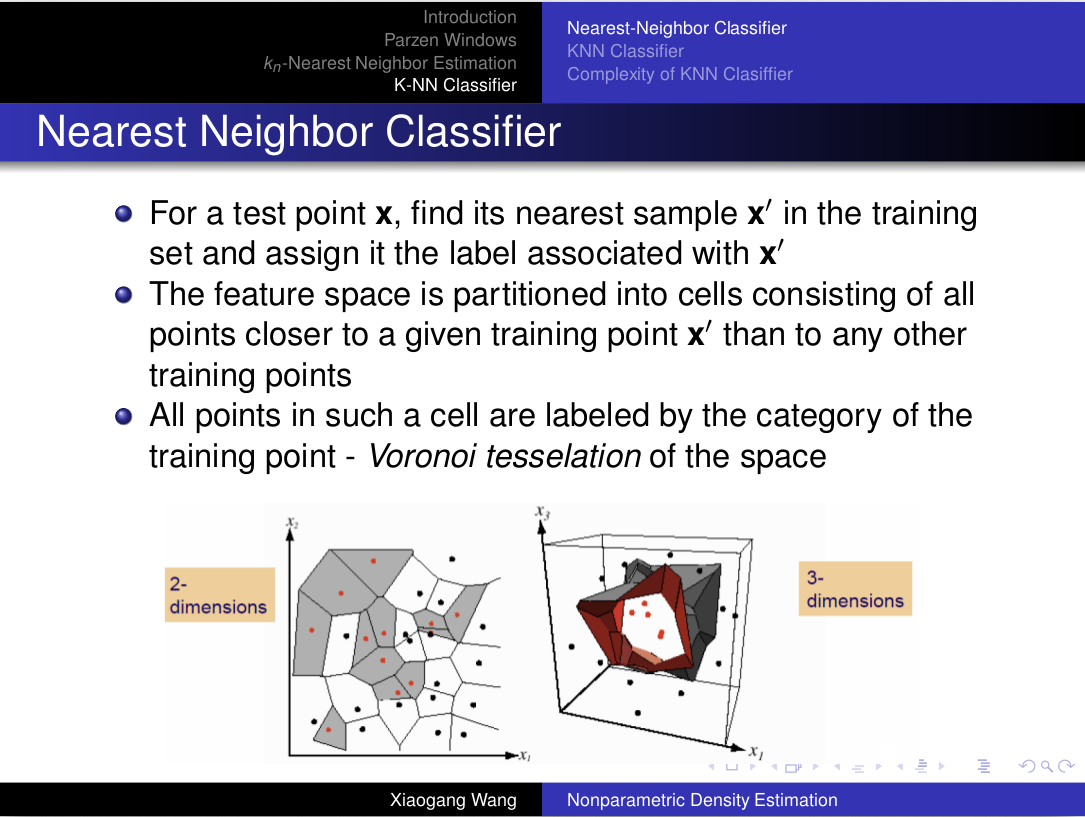
\includegraphics[width=\paperwidth]{figures/ex1.png}
            };
        \end{tikzpicture}
     \end{frame}
}

\begin{frame}{Ex.1: Voronoi cell}
	\begin{block}{Problem}
		Prove that the Voronoi cells induced by the single-nearest neighbor algorithm
		must always be convex. That is, for any two points $x_1$ and $x_2$ in a cell, all points on the line linking $x_1$ and $x_2$ must also lie in the cell.
	\end{block}
\end{frame}

\begin{frame}{Ex.1: Voronoi cell}
	\scriptsize
	\begin{block}{Solution}
		Our goal is to show that Voronoi cells induced by the nearest-neighbor algorithm are convex, that is, given any two points in the cell, the line connecting them also lies in the cell. We let $x^*$ be the labeled sample point in the Voronoi cell, and $y$ be any other labeled sample point. A unique hyperplane separates the space into those that are closer to $x^*$ than to y, as shown in the figure. Consider any two points $x_0$ and $x_1$ inside the Voronoi cell of $x^*$; these points are surely on the side of the hyperplane nearest $x^*$. Now consider the line connecting those points, parameterized as $x(\lambda) = (1-\lambda)x_0 + \lambda x_1$ for $0\leq \lambda \leq 1$. Because the half-space defined by the hyperplane is convex, all the points $x(\lambda)$ lie nearer to $x^*$ than to $y$. This is true for every other sample point $y_i$. Thus $x(\lambda)$ remains closer to $x^*$ than any other labeled point. By our definition of convexity, we have, then, that the Voronoi cell is convex. 
	\end{block}
	\centering
	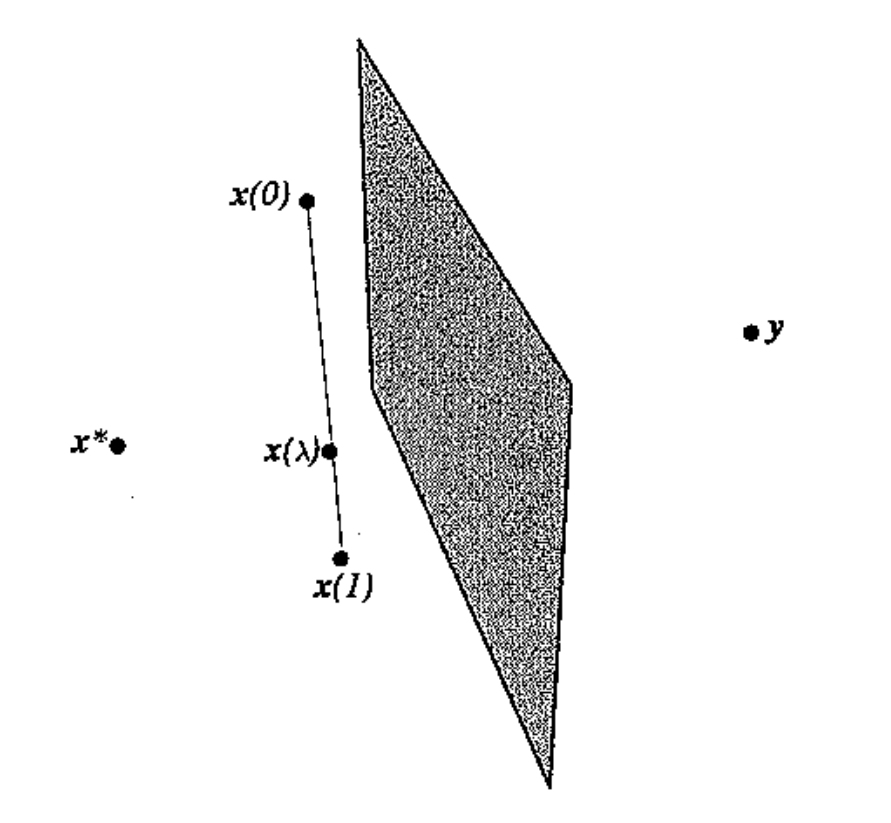
\includegraphics[width=0.35\linewidth]{figures/ex1s.png}
\end{frame}

\begin{frame}{Outline}
\setbeamercovered{transparent}
	\begin{enumerate}
		\item<0> Ex.1: Voronoi cell
		\vspace{0.1in}
		\item<1> Ex. 2: Nearest neighor error v.s. Bayes error
	\end{enumerate}
\end{frame}

{ % all template changes are local to this group.
    \setbeamertemplate{navigation symbols}{}
    \begin{frame}[plain]
        \begin{tikzpicture}[remember picture,overlay]
            \node[at=(current page.center)] {
                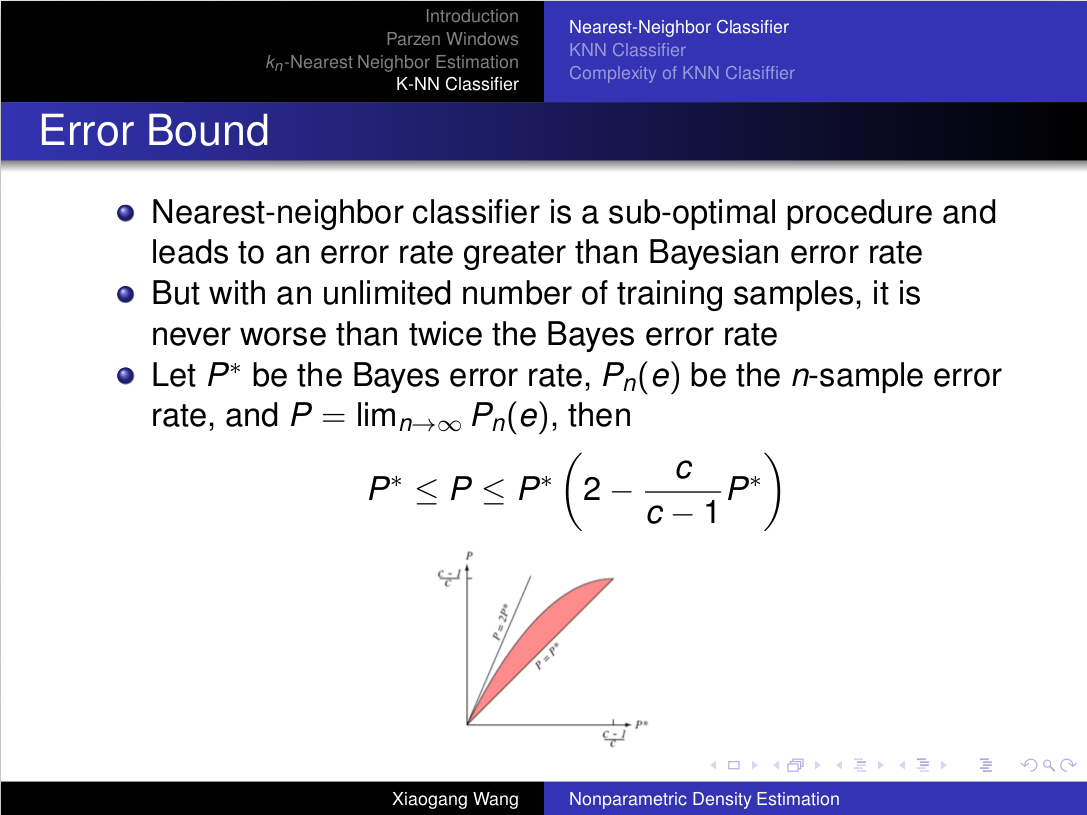
\includegraphics[width=\paperwidth]{figures/ex2.png}
            };
        \end{tikzpicture}
     \end{frame}
}

\begin{frame}{Ex.2: Nearest neighbor error rate}
	\begin{block}{Review}
		\small
		Independently drawn labelled samples:
		\begin{align}
			(x_1, \theta_1), (x_2, \theta_2), \hdots, (x_n, \theta_n),
		\end{align}
		where $\theta_j$ may be any of $c$ states of nature $w_i, i = 1, ..., c$.
		Given a test $(x, \theta)$, its nearest training sample is $x_{nn}$, we have
		\begin{align}
			P(\theta, \theta_{nn} | x, x_{nn}) = P(\theta | x) P(\theta_{nn} | x_{nn})
		\end{align}
		The nearest-neighbor decision rule: commit an error whenever $\theta \neq \theta_{nn}$
		\begin{align}
			P_n(e | x, x_{nn}) &= 1 - \sum_{i=1}^c P(\theta = w_i, \theta_{nn} = w_i | x, x_{nn}) \\
			&=1 - \sum_{i=1}^c P(\theta = w_i|x)P(\theta_{nn} = w_i | x_{nn})
		\end{align}
		\normalsize
	\end{block}
\end{frame}

\begin{frame}{Ex.2: Nearest neighbor error rate}
	\begin{block}{Review [continue]}
		\begin{align}
			p(e|x) = \int P(e | x, x_{nn}) p(x_{nn} | x) dx_{nn}
		\end{align}
		where $~~p(x_{nn} | x) \rightarrow \delta(x_{nn} - x),~~ n \rightarrow \infty$, \\
		and $~~P_n(e | x, x_{nn}) = 1 - \sum_{i=1}^c P(\theta = w_i|x)P(\theta_{nn} = w_i | x_{nn})$ 
		Thus, 
		\begin{align}
			p(e|x) = \lim_{n\rightarrow \infty} P_n(e|x) &= \int P_n(e | x, x_{nn}) \delta(x_{nn} - x) dx_{nn}\\
			& = 1 - \sum_{i=1}^c P^2(\theta = w_i|x)
		\end{align}
	\end{block}
\end{frame}

\begin{frame}{Ex.2: Nearest neighor error v.s. Bayes error}
	\begin{block}{Problem}
		It is easy to see that the nearest-neighbor error rate $P$ can equal the Bayes rate $P^*$ if $P^*=0$ (the best possibility) or if $P^* = \frac{c-1}{c}$ (the worst possibility). One might ask whether or not there are problems for which $P=P^*$ when $P$ is between these extremes. 
		\begin{enumerate}
			\item Show that the Bayes rate for the one-dimensional case where $P(w_i) = 1/c$ and 
			\begin{align}
				P(x|w_i) = \left\{ 
				\begin{tabular}{ll}
				1 & $0\leq x\leq \frac{cr}{c-1}$ \\
				1 & $i\leq x \leq i + 1-\frac{cr}{c-1}$ \\
				0 & otherwise
				\end{tabular}
				\right.
			\end{align}
			is $P^* = r$.
			\item Show that for this case that the nearest-neighbor rate is $P=P^*$.
		\end{enumerate}
	\end{block}
\end{frame}

\begin{frame}{Ex.2: Nearest neighor error v.s. Bayes error}
	\begin{block}{Solution}
		It is indeed possible to have the nearest-neighbor error rate $P$ equal to the Bayes error rate $P^*$ for non-trivial distribution. 
		\begin{enumerate}
			\item Consider uniform priors over c categories, that is, $P(w_i) = 1/c$, and one-dimensional distributions
			\begin{align}
				P(x|w_i) = \left\{ 
				\begin{tabular}{ll}
				1 & $0\leq x\leq \frac{cr}{c-1}$ \\
				1 & $i\leq x \leq i + 1-\frac{cr}{c-1}$ \\
				0 & otherwise
				\end{tabular}
				\right.
			\end{align}
			Note that this automatically impose the restriction
			\begin{align}
				0 \leq \frac{cr}{c-1} \leq 1
			\end{align}
			
		\end{enumerate}
	\end{block}
\end{frame}

\begin{frame}{Ex.2: Nearest neighor error v.s. Bayes error}
	\begin{block}{Solution [continue]}
		\begin{enumerate}
			\item The evidence is 
			\begin{align}
				p(x) = \Sigma_{i=1}^c p(x|w_i)P(w_i) = \left\{ 
				\begin{tabular}{ll}
				1 & $0\leq x\leq \frac{cr}{c-1}$ \\
				1/c & $i\leq x \leq i + 1-\frac{cr}{c-1}$ \\
				0 & otherwise
				\end{tabular}
				\right.
			\end{align}
			Because the $P(w_i)$ are constant, we have $P(w_i|x) \propto p(x|w_i)$ and thus 
			\begin{align}
				P(w_i | x) = \left\{ 
				\begin{tabular}{ll}
				$\frac{P(w_i)}{p(x)} = \frac{1/c}{p(x)}$ & $0\leq x\leq \frac{cr}{c-1}$ \\
				\begin{tabular}{ll} 
				0 & if $i \neq j$ \\ 
				1 & if $ i = j $
				\end{tabular}\Big\} 
				&
				$j\leq x \leq j + 1-\frac{cr}{c-1}$ \\
				0 & otherwise
				\end{tabular}
				\right.
			\end{align}
		\end{enumerate}
	\end{block}
\end{frame}

\begin{frame}{Ex.2: Nearest neighor error v.s. Bayes error}
	\begin{block}{Solution [continue]}
		\begin{enumerate}
			\item The conditional Bayesian probability of error at a point $x$ is 
			\begin{align}
				P^*(e|x) & = 1-P(w_{\max} |x) \\
				& = \left\{ 
				\begin{tabular}{ll}
				$1- \frac{1/c}{p(x)}$ & if $0 \leq x \leq \frac{cr}{c-1}$ \\
				$1 - 1 = 0$ & if $i \leq x \leq i+1-\frac{cr}{c-1}$
				\end{tabular}\right.
			\end{align}
			and to calculate the full Bayes probability of error, we integrate as 
			\vspace{-0.1in}
			\begin{align}
				P^* &= \int P^*(e|x)p(x) dx \\
				& = \int_{0}^{cr/(c-1)} \Big[1 - \frac{1/c}{p(x)}\Big] p(x)dx \\
				& = \big(1 - \frac{1}{c}\big) \frac{cr}{c-1} = r.
			\end{align}
		\end{enumerate}
	\end{block}
\end{frame}

\begin{frame}{Ex.2: Nearest neighor error v.s. Bayes error}
	\begin{block}{Solution [continue]}
		\small
		\begin{enumerate}
			\item<0> \vspace{-0.2in}
			\item The nearest-neighbor error rate is 
			\begin{align}
				P & = \int p(e|x) p(x) dx \\
				& = \int \Big[1-\sum_{i=1}^c P^2(w_i | x)\Big] p(x) dx \\
				& = \int_0^{cr/(c-1)}\Big[1 - \frac{c(\frac{1}{c})^2}{p^2(x)}\Big]p(x)dx + \sum_{j=1}^c\int_j^{j+1-\frac{cr}{c-1}}[1-1]p(x)dx \nonumber\\
				& = \int_0^{cr/(c-1)} \Big(1 - \frac{1/c}{p^2(x)}\Big)p(x)dx \\
				& = \int_0^{cr/(c-1)} \Big(1 - \frac{1}{c}\Big)dx = \Big(1-\frac{1}{c}\Big)\frac{cr}{c-1} = r.
			\end{align}
			Thus we have demonstrated that $P^* = P = r$ in this nontrivial case.
		\end{enumerate}
		\normalsize
	\end{block}
\end{frame}

\begin{frame}{Reference on Nearest Neighbor Error Bound}
	\begin{enumerate}
		\item Cover, Thomas, and Peter Hart. Nearest neighbor pattern classification. IEEE Transactions on Information Theory, 1967.
		\item Duda, Richard O., Peter E. Hart, and David G. Stork. Pattern classification. 2012.
	\end{enumerate}
\end{frame}

\end{document} 